\documentclass[aspectratio=169]{beamer}
\usetheme{default}
\usefonttheme{professionalfonts}
\usepackage{graphicx}
\usepackage{booktabs}
\usepackage{array}
\graphicspath{{../assets/}{../visualizations/}{./}}

% Palette
\definecolor{Ink}{HTML}{1A1C1E}
\definecolor{Navy}{HTML}{16324F}
\definecolor{Teal}{HTML}{1E6B5E}
\definecolor{Amber}{HTML}{A76F00}
\definecolor{Mist}{HTML}{F2F5F7}
\definecolor{Steel}{HTML}{5C6B7A}
\definecolor{Warn}{HTML}{8A2C2C}

% Beamer colours
\setbeamercolor{normal text}{fg=Ink,bg=white}
\setbeamercolor{structure}{fg=Navy}
\setbeamercolor{frametitle}{fg=white,bg=Navy}
\setbeamercolor{title}{fg=Navy}
\setbeamercolor{subtitle}{fg=Amber}
\setbeamercolor{block title}{fg=white,bg=Teal}
\setbeamercolor{block body}{fg=Ink,bg=Mist}
\setbeamercolor{alerted text}{fg=Warn}
\setbeamercolor{itemize item}{fg=Amber}
\setbeamercolor{itemize subitem}{fg=Teal}

% Templates
\setbeamertemplate{navigation symbols}{}
\setbeamertemplate{itemize item}{\small\color{Amber}$\triangleright$}
\setbeamertemplate{itemize subitem}{\small\color{Teal}--}
\setbeamertemplate{enumerate item}{\color{Navy}\insertenumlabel.}
\setbeamertemplate{frametitle}{
  \nointerlineskip
  \begin{beamercolorbox}[wd=\paperwidth,ht=2.6ex,dp=1ex,leftskip=0.5cm]{frametitle}
    \usebeamerfont{frametitle}\insertframetitle
  \end{beamercolorbox}
  \vspace{-1pt}
  {\color{Amber}\hrule height 1.4pt}
}
\setbeamertemplate{footline}{
  \leavevmode\hbox{%
    \begin{beamercolorbox}[wd=.72\paperwidth,ht=2ex,dp=0.75ex,leftskip=0.4cm]{author in head/foot}
      \color{Steel}\tiny CS343 Graph Data Science \textbf{.} POLE Crime Investigation
    \end{beamercolorbox}
    \begin{beamercolorbox}[wd=.28\paperwidth,ht=2ex,dp=0.75ex,rightskip=0.4cm plus1fil]{date in head/foot}
      \color{Steel}\tiny\hfill\insertframenumber\,/\,\inserttotalframenumber
    \end{beamercolorbox}}
}
\setbeamertemplate{title page}{
  \vfill
  \begin{beamercolorbox}[leftskip=0.8cm,rightskip=0.8cm]{title}
    {\usebeamerfont{title}\Large\textbf{\inserttitle}\par}
    \vspace{0.2cm}
    {\color{Amber}\rule{0.76\paperwidth}{1.5pt}\par}
    \vspace{0.2cm}
    {\usebeamerfont{subtitle}\normalsize\insertsubtitle\par}
    \vspace{0.45cm}
    {\small\color{Steel}\insertauthor\par}
    \vspace{0.1cm}
    {\footnotesize\color{Steel}\insertinstitute\quad|\quad\insertdate\par}
  \end{beamercolorbox}
  \vfill
}

\renewcommand{\arraystretch}{1.12}
\newcommand{\tinycode}[1]{\texttt{\scriptsize #1}}

% Meta
\title{POLE Crime Investigation with Graph Data Science}
\subtitle{From sparse prediction targets to explainable investigative prioritization}
\author{Amn Naqvi \quad\&\quad Rayyan Shah}
\institute{CS343 Graph Data Science \quad|\quad Project Group 4}
\date{Spring 2026}

\begin{document}

\begin{frame}
  \titlepage
\end{frame}

\begin{frame}{Demo Roadmap}
  \begin{enumerate}
    \item Project problem and scope.
    \item POLE graph model and database size.
    \item Graph stats results: structure, relationship coverage, and analytics.
    \item Link viability audit: which relationships are actually strong.
    \item Graph ML pipeline: supervised and explainable link prediction.
    \item Metrics, calibration, course deliverables, and final demo conclusion.
  \end{enumerate}
\end{frame}

\begin{frame}{Problem Statement}
  \textbf{Question:} How can a POLE crime graph support investigative review without overstating what the data can prove?

  \vspace{0.3cm}
  \begin{columns}[T]
    \column{0.48\textwidth}
      \textbf{Original temptation}
      \begin{itemize}
        \item Predict \tinycode{Person -> Crime}.
        \item Treat \tinycode{PARTY\_TO} as the main ML target.
        \item Write back likely crime links.
      \end{itemize}

    \column{0.48\textwidth}
      \textbf{Final research framing}
      \begin{itemize}
        \item Find hotspots and repeat place patterns.
        \item Detect social communities and review-priority people.
        \item Use GML for review-only social link candidates.
        \item Block automated person-crime write-back when the data does not justify it.
      \end{itemize}
  \end{columns}
\end{frame}

\begin{frame}{Project Scope from the Brief}
  The course brief asks for graph model design, graph statistics, graph analytics, and graph machine learning.

  \vspace{0.25cm}
  \begin{table}
    \centering\small
    \begin{tabular}{p{0.24\textwidth}p{0.62\textwidth}}
      \toprule
      \textbf{Requirement} & \textbf{What this project demonstrates} \\
      \midrule
      Graph model/loading & POLE graph restored from Neo4j dump with people, crimes, locations, vehicles, phones, officers, areas. \\
      Graph statistics & Node counts, relationship counts, degree distribution, isolated nodes, target density. \\
      Graph analytics & Hotspots, crime-type profiles, Louvain communities, WCC, k-core structure, and contextual review scores. \\
      Graph ML & GDS social-family link prediction, explainable Common Neighbours, Adamic Adar, kNN similarity, and crime-type classification. \\
      Critical analysis & Person-Crime prediction tested and rejected as a main deployment target because labels are sparse and sensitive. \\
      \bottomrule
    \end{tabular}
  \end{table}
\end{frame}

\begin{frame}{Final Demo Alignment}
  \small
  \begin{table}
    \centering
    \begin{tabular}{p{0.28\textwidth}p{0.56\textwidth}}
      \toprule
      \textbf{Demo expectation} & \textbf{What we will show live} \\
      \midrule
      Graph model and database & POLE schema, node labels, relationship types, and graph size: 61,521 nodes and 105,840 relationships. \\
      Key analytics and queries & Link viability audit, hotspot locations, dominant crime-type profiles, Louvain communities, k-core/WCC structure, and review-priority context. \\
      GML pipeline and results & FastRP + Node2Vec + Logistic Regression/Random Forest social-family link prediction, AUCPR metrics, deployment gate, and explainable social-link candidates. \\
      Comparative insight & Graph methods expose paths, communities, and shared neighbours; direct person-crime prediction is rejected because \tinycode{PARTY\_TO} has only 55 labels. \\
      Responsible interpretation & Every person-level output is review-only. No automated crime claim is written back. \\
      \bottomrule
    \end{tabular}
  \end{table}
\end{frame}

\begin{frame}{POLE Graph Model}
  \begin{columns}[T]
    \column{0.52\textwidth}
      \begin{center}
        \IfFileExists{POLE.jpeg}{
          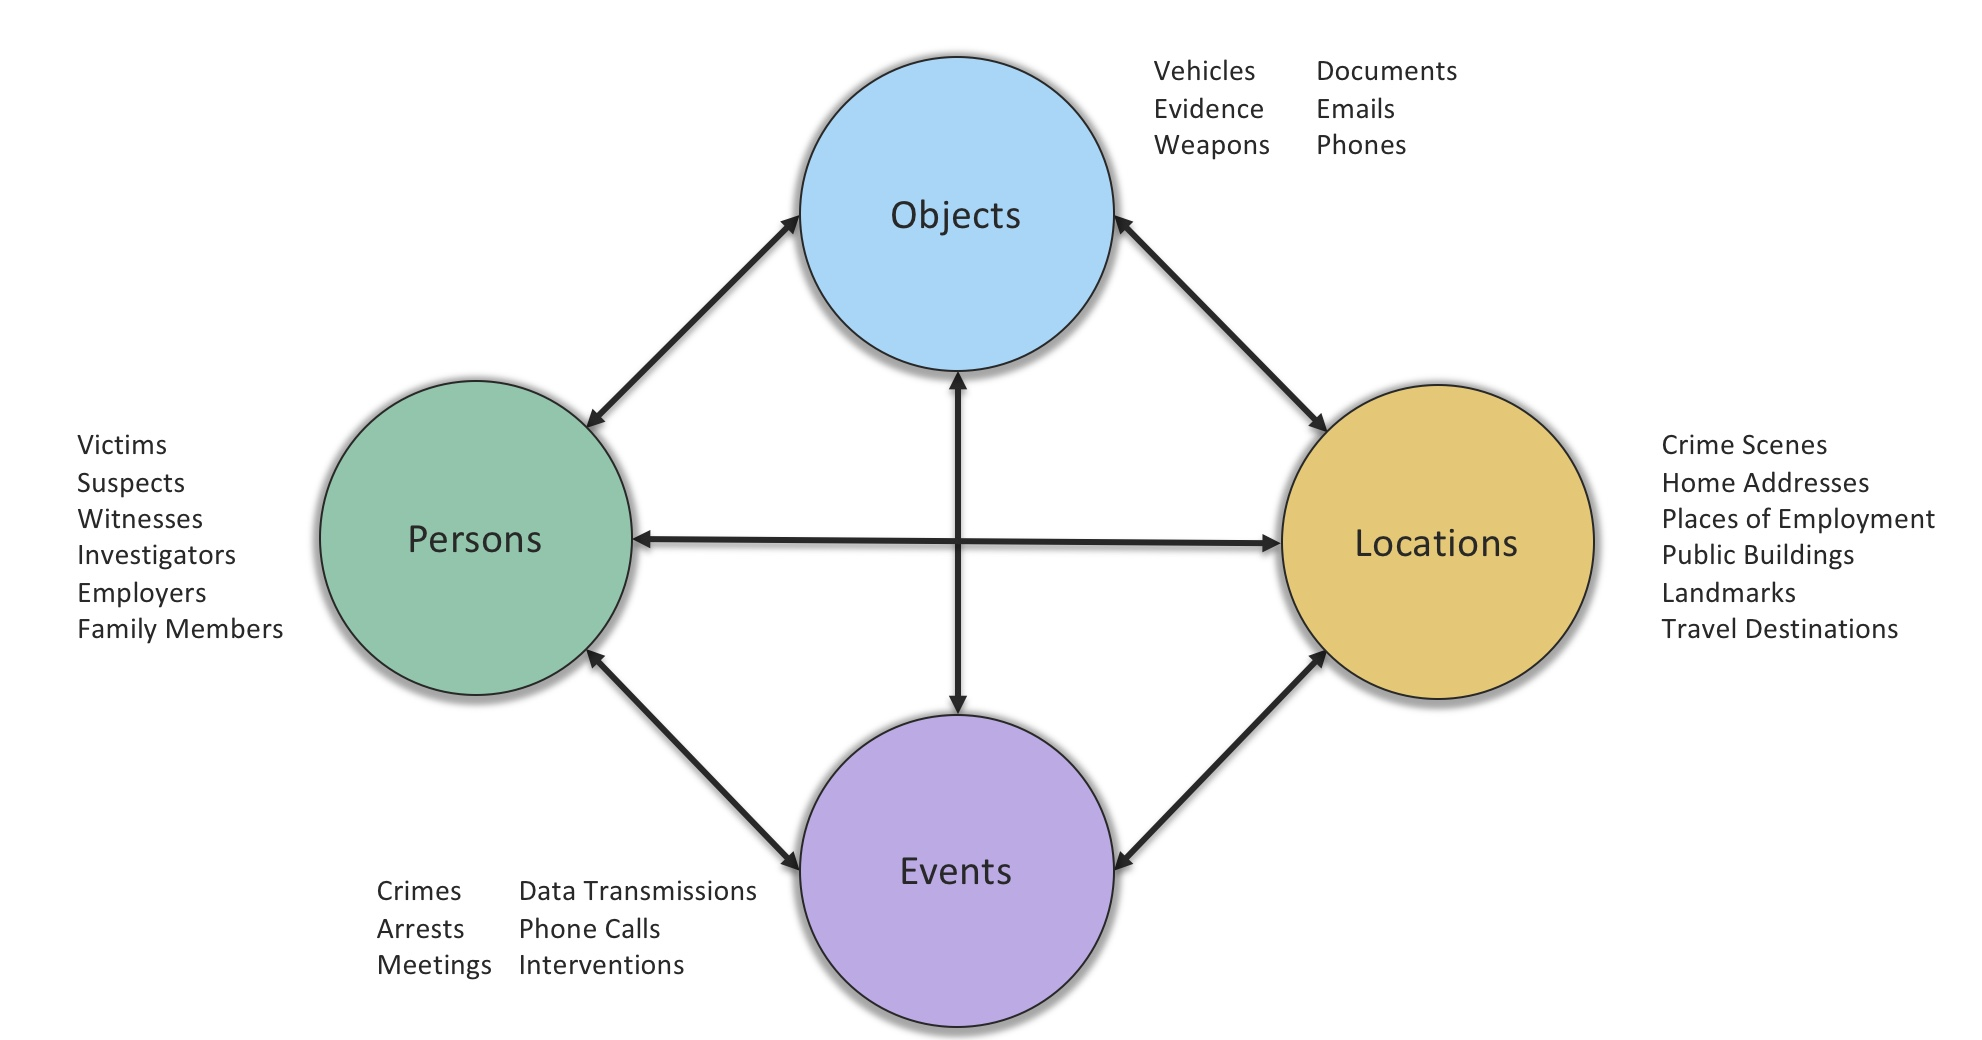
\includegraphics[width=0.96\textwidth,height=0.62\textheight,keepaspectratio]{POLE.jpeg}
        }{
          \fbox{\begin{minipage}[c][0.58\textheight][c]{0.9\textwidth}
            \centering\color{Steel}POLE.jpeg
          \end{minipage}}
        }
      \end{center}

    \column{0.44\textwidth}
      \textbf{Core idea}
      \begin{itemize}
        \item Persons, Objects, Locations, and Events are not isolated tables.
        \item Crimes connect to places.
        \item People connect through social, address, phone, and observed crime context.
        \item Graph paths give explanations that flat tables hide.
      \end{itemize}
  \end{columns}
\end{frame}

\begin{frame}{Database Snapshot}
  \begin{columns}[T]
    \column{0.47\textwidth}
      \textbf{Overall graph}\\[4pt]
      \small
      \begin{tabular}{lr}
        \toprule
        \textbf{Metric} & \textbf{Value} \\
        \midrule
        Total nodes & 61,521 \\
        Total relationships & 105,840 \\
        Average degree & 3.4408 \\
        Maximum degree & 1,321 \\
        Isolated persons & 1 \\
        \bottomrule
      \end{tabular}

    \column{0.50\textwidth}
      \textbf{Important labels}\\[4pt]
      \small
      \begin{tabular}{lr}
        \toprule
        \textbf{Label} & \textbf{Count} \\
        \midrule
        Crime & 28,762 \\
        Location & 14,904 \\
        PostCode & 14,196 \\
        Officer & 1,000 \\
        Vehicle & 1,000 \\
        Person & 369 \\
        Object & 7 \\
        \bottomrule
      \end{tabular}
  \end{columns}
\end{frame}

\begin{frame}{Visual Snapshot: Graph Scale}
  \begin{columns}[T]
    \column{0.49\textwidth}
      \centering
      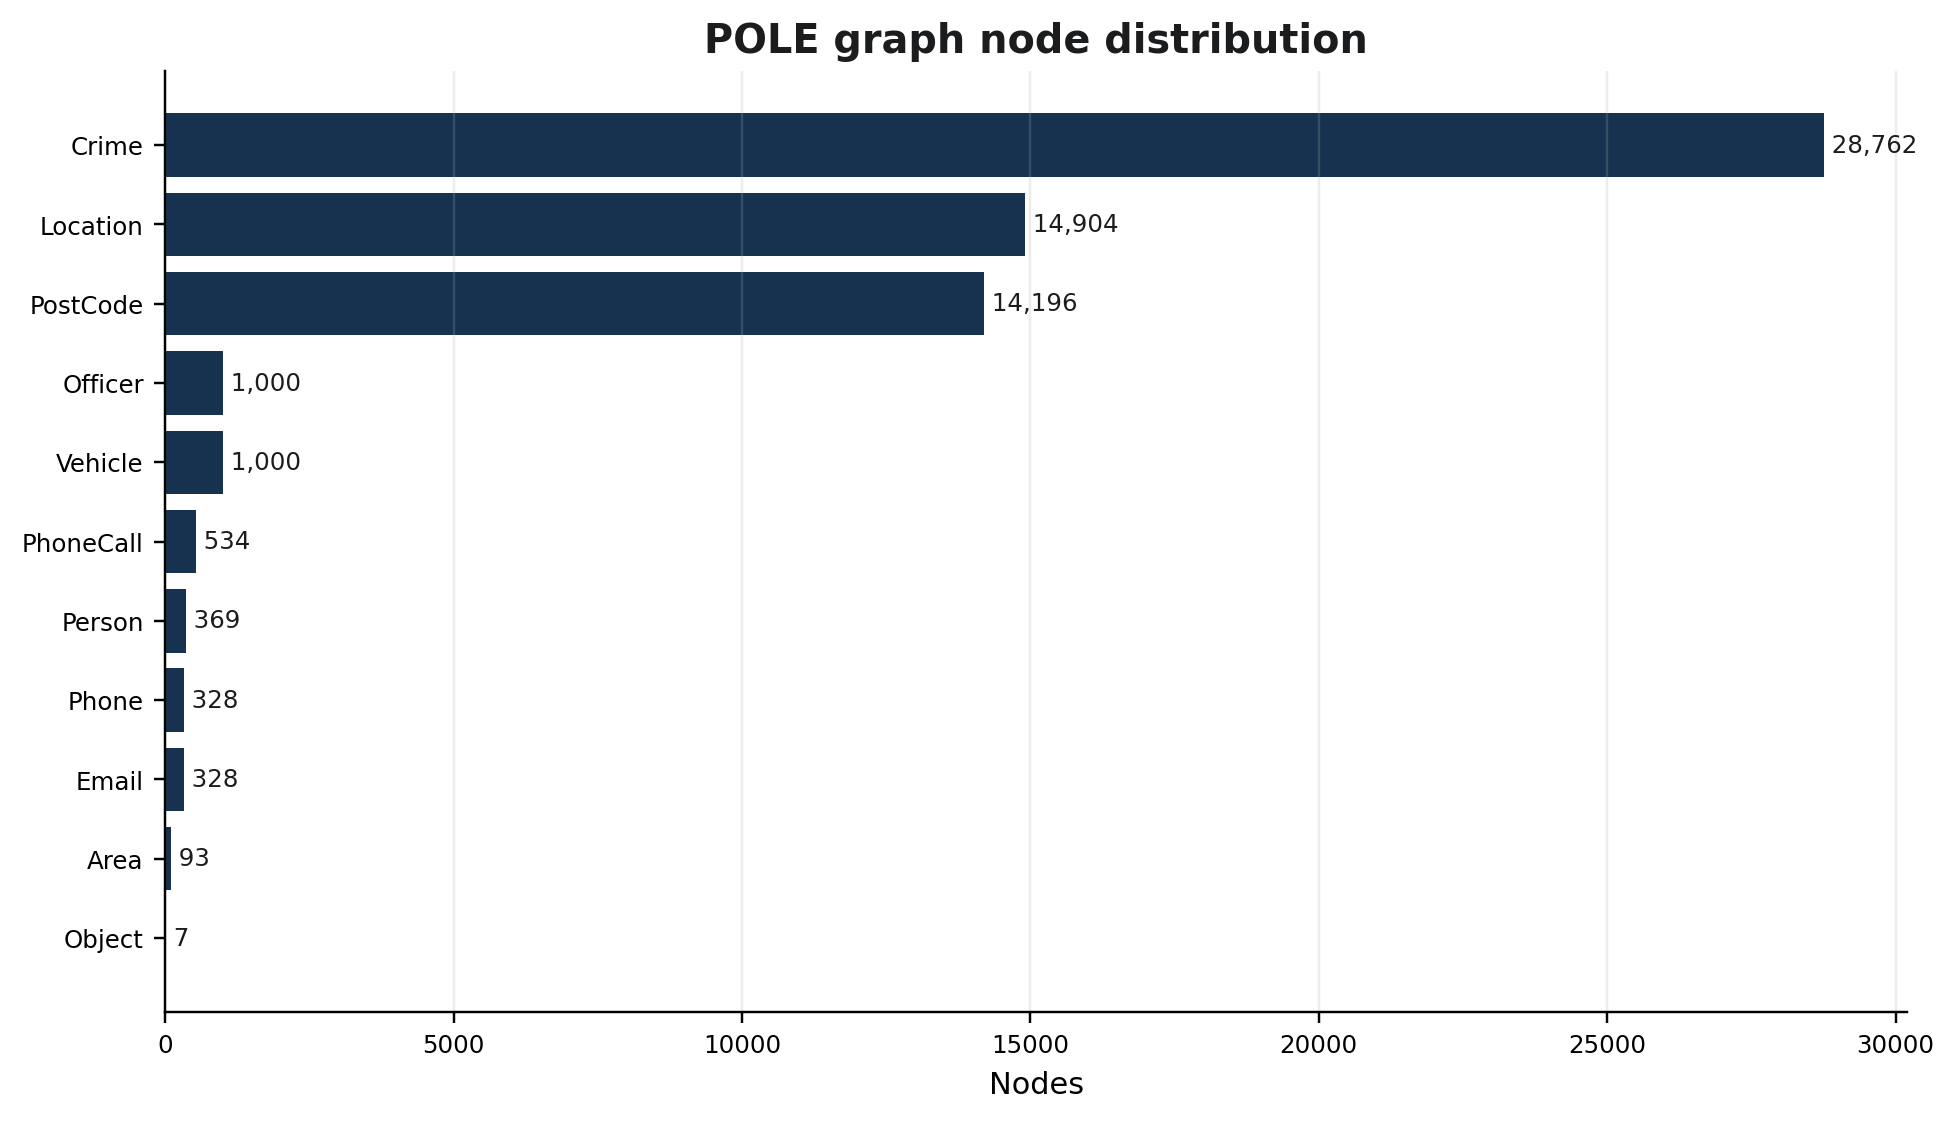
\includegraphics[width=\textwidth,height=0.72\textheight,keepaspectratio]{01_node_distribution.png}

    \column{0.49\textwidth}
      \centering
      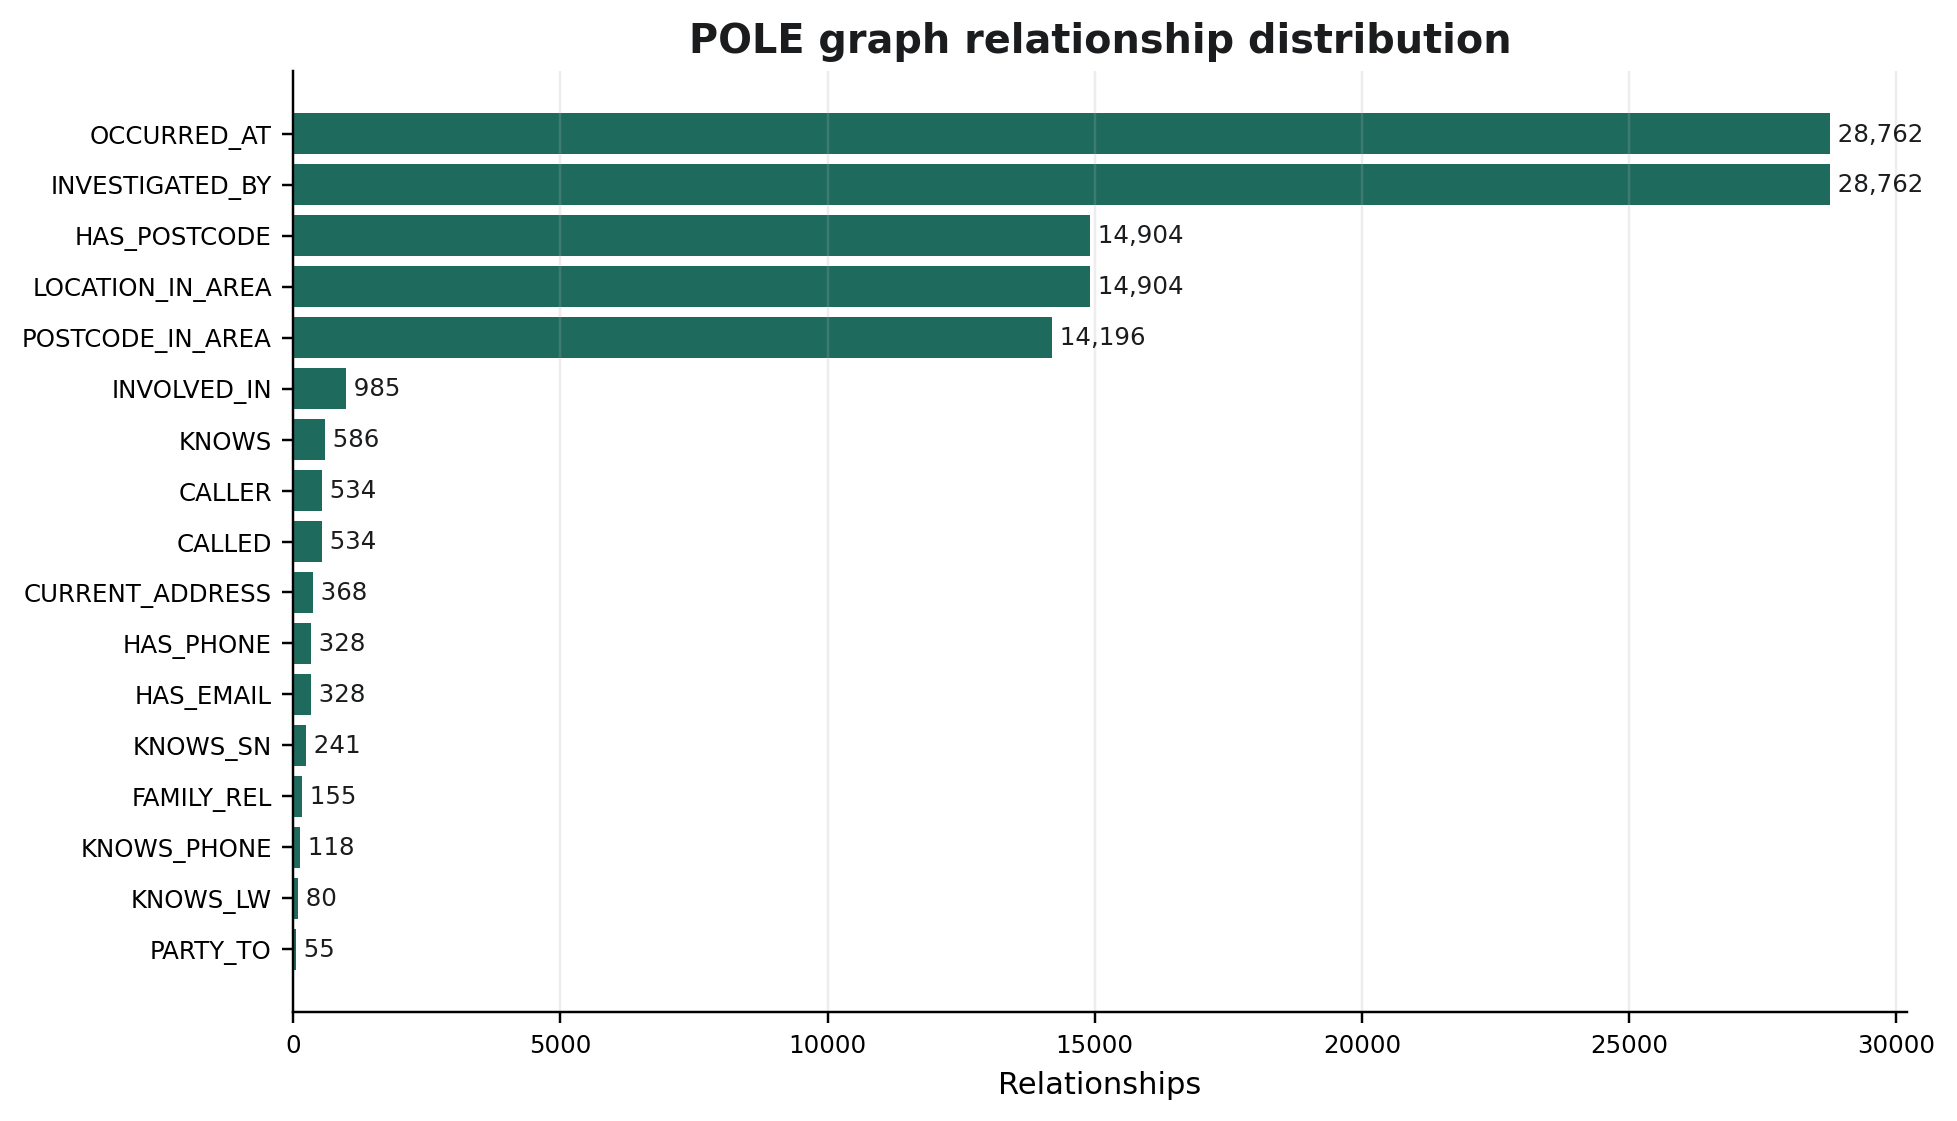
\includegraphics[width=\textwidth,height=0.72\textheight,keepaspectratio]{02_relationship_distribution.png}
  \end{columns}
  \vspace{0.1cm}
\end{frame}

\begin{frame}{Link Viability Audit}
  \small
  \begin{table}
    \centering
    \begin{tabular}{p{0.22\textwidth}r p{0.48\textwidth}}
      \toprule
      \textbf{Link family} & \textbf{Links} & \textbf{Final reading} \\
      \midrule
      Crime $\rightarrow$ Location & 28,762 & Strongest signal: complete crime coverage and clear hotspot interpretation. \\
      Person $\rightarrow$ Person & 1,180 raw links & Strong GDS surface for communities; collapsed to 586 unique undirected social-family pairs for supervised link prediction. \\
      PhoneCall $\rightarrow$ Phone & 1,068 & Useful context, but not the main target. \\
      Vehicle $\rightarrow$ Crime & 978 & Useful context; mostly one-off vehicle-crime links. \\
      Person $\rightarrow$ Location & 368 & Address exposure context, not proof. \\
      Person $\rightarrow$ Crime & 55 & Too sparse and sensitive to carry the main prediction task. \\
      Object $\rightarrow$ Crime & 7 & Too small for meaningful modelling. \\
      \bottomrule
    \end{tabular}
  \end{table}
\end{frame}

\begin{frame}{Graph Stats Result: Hotspot Analytics}
  \small
  \begin{table}
    \centering
    \begin{tabular}{lrrl}
      \toprule
      \textbf{Location} & \textbf{Incidents} & \textbf{Crime types} & \textbf{Priority} \\
      \midrule
      Parking Area & 811 & 13 & Very high \\
      Supermarket & 614 & 13 & Very high \\
      Shopping Area & 594 & 13 & Very high \\
      Nightclub & 336 & 13 & High \\
      Petrol Station & 331 & 13 & High \\
      Sports/Recreation Area & 169 & 12 & High \\
      Piccadilly & 166 & 11 & High \\
      \bottomrule
    \end{tabular}
  \end{table}

  \vspace{0.15cm}
  \textbf{Demo query:} \tinycode{MATCH (c:Crime)-[:OCCURRED\_AT]->(l:Location) RETURN l.address, count(c)}
\end{frame}

\begin{frame}{Visual Snapshot: Hotspots and Link Viability}
  \begin{columns}[T]
    \column{0.49\textwidth}
      \centering
      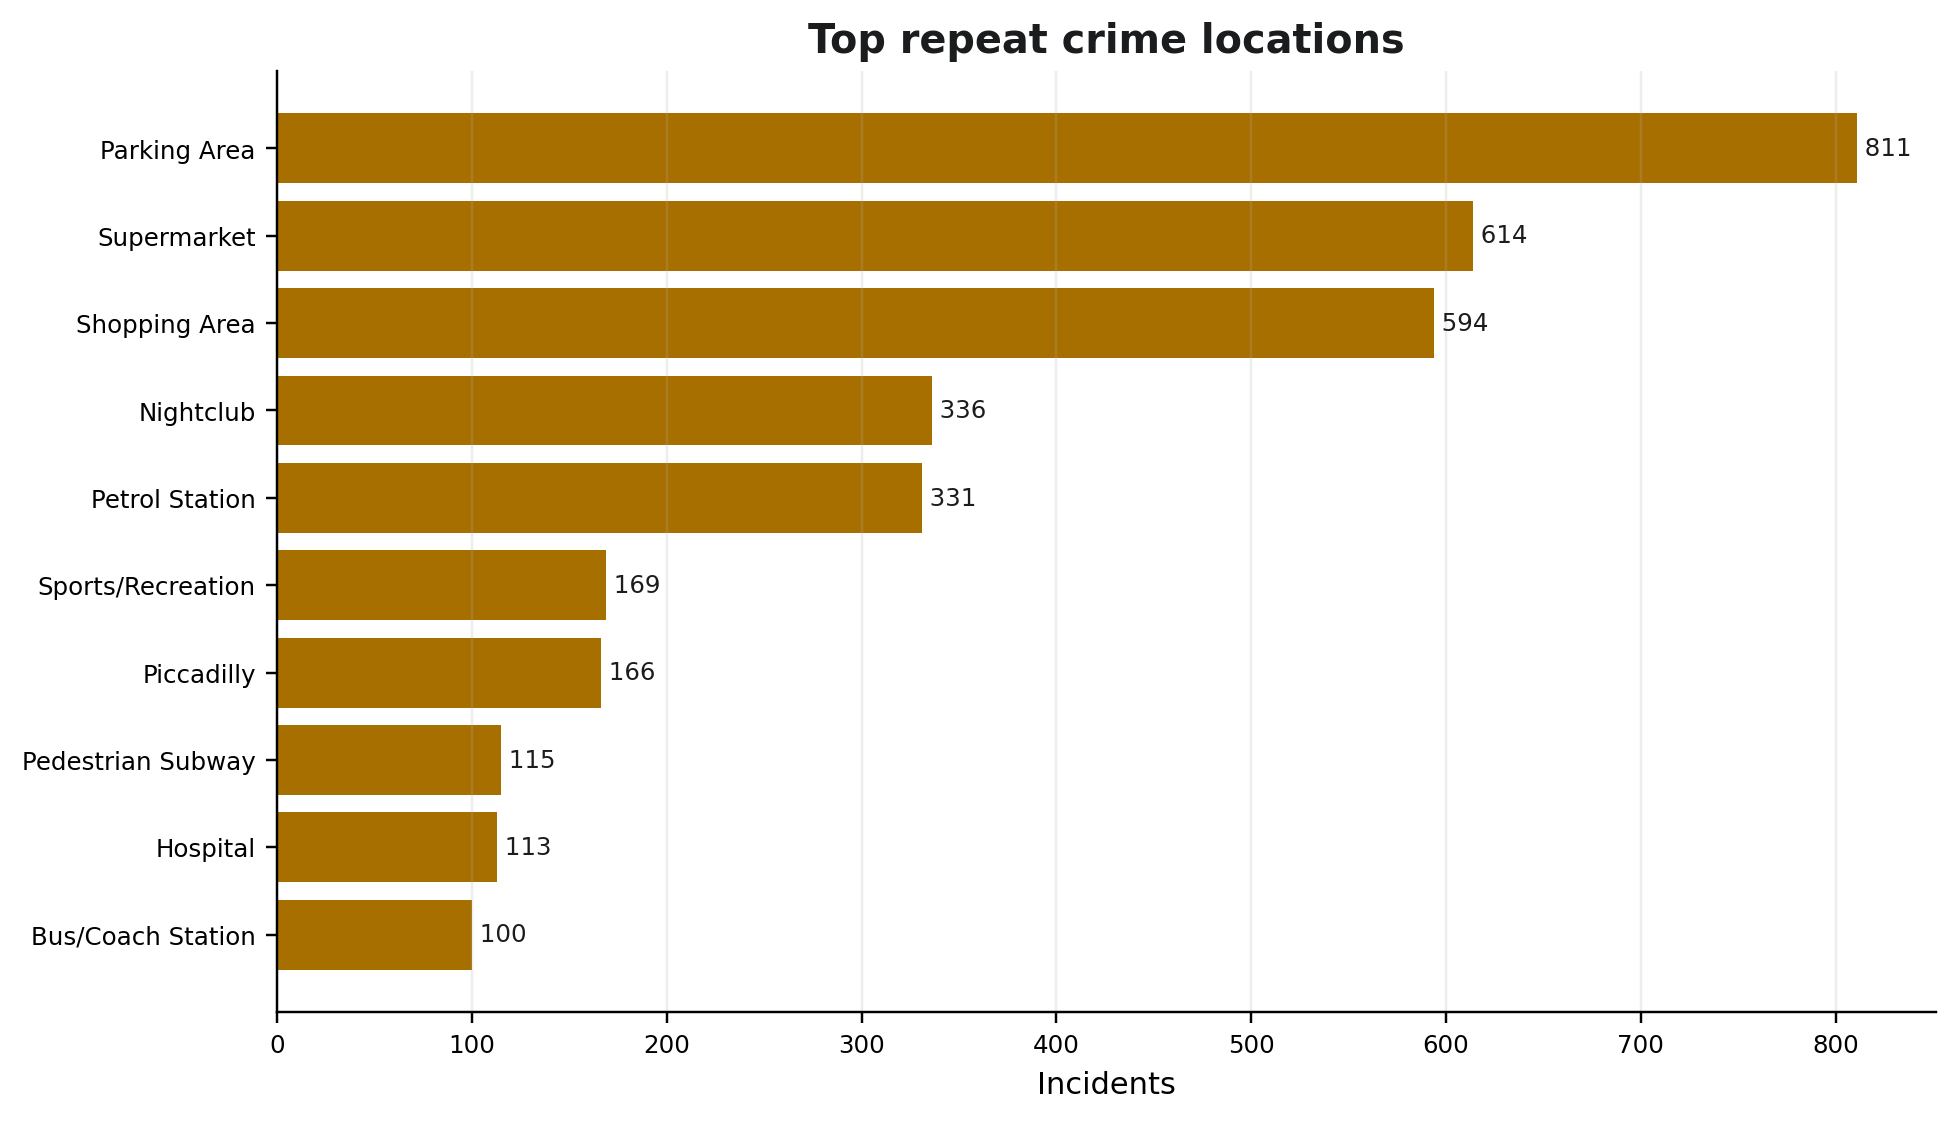
\includegraphics[width=\textwidth,height=0.72\textheight,keepaspectratio]{03_top_hotspots.png}

    \column{0.49\textwidth}
      \centering
      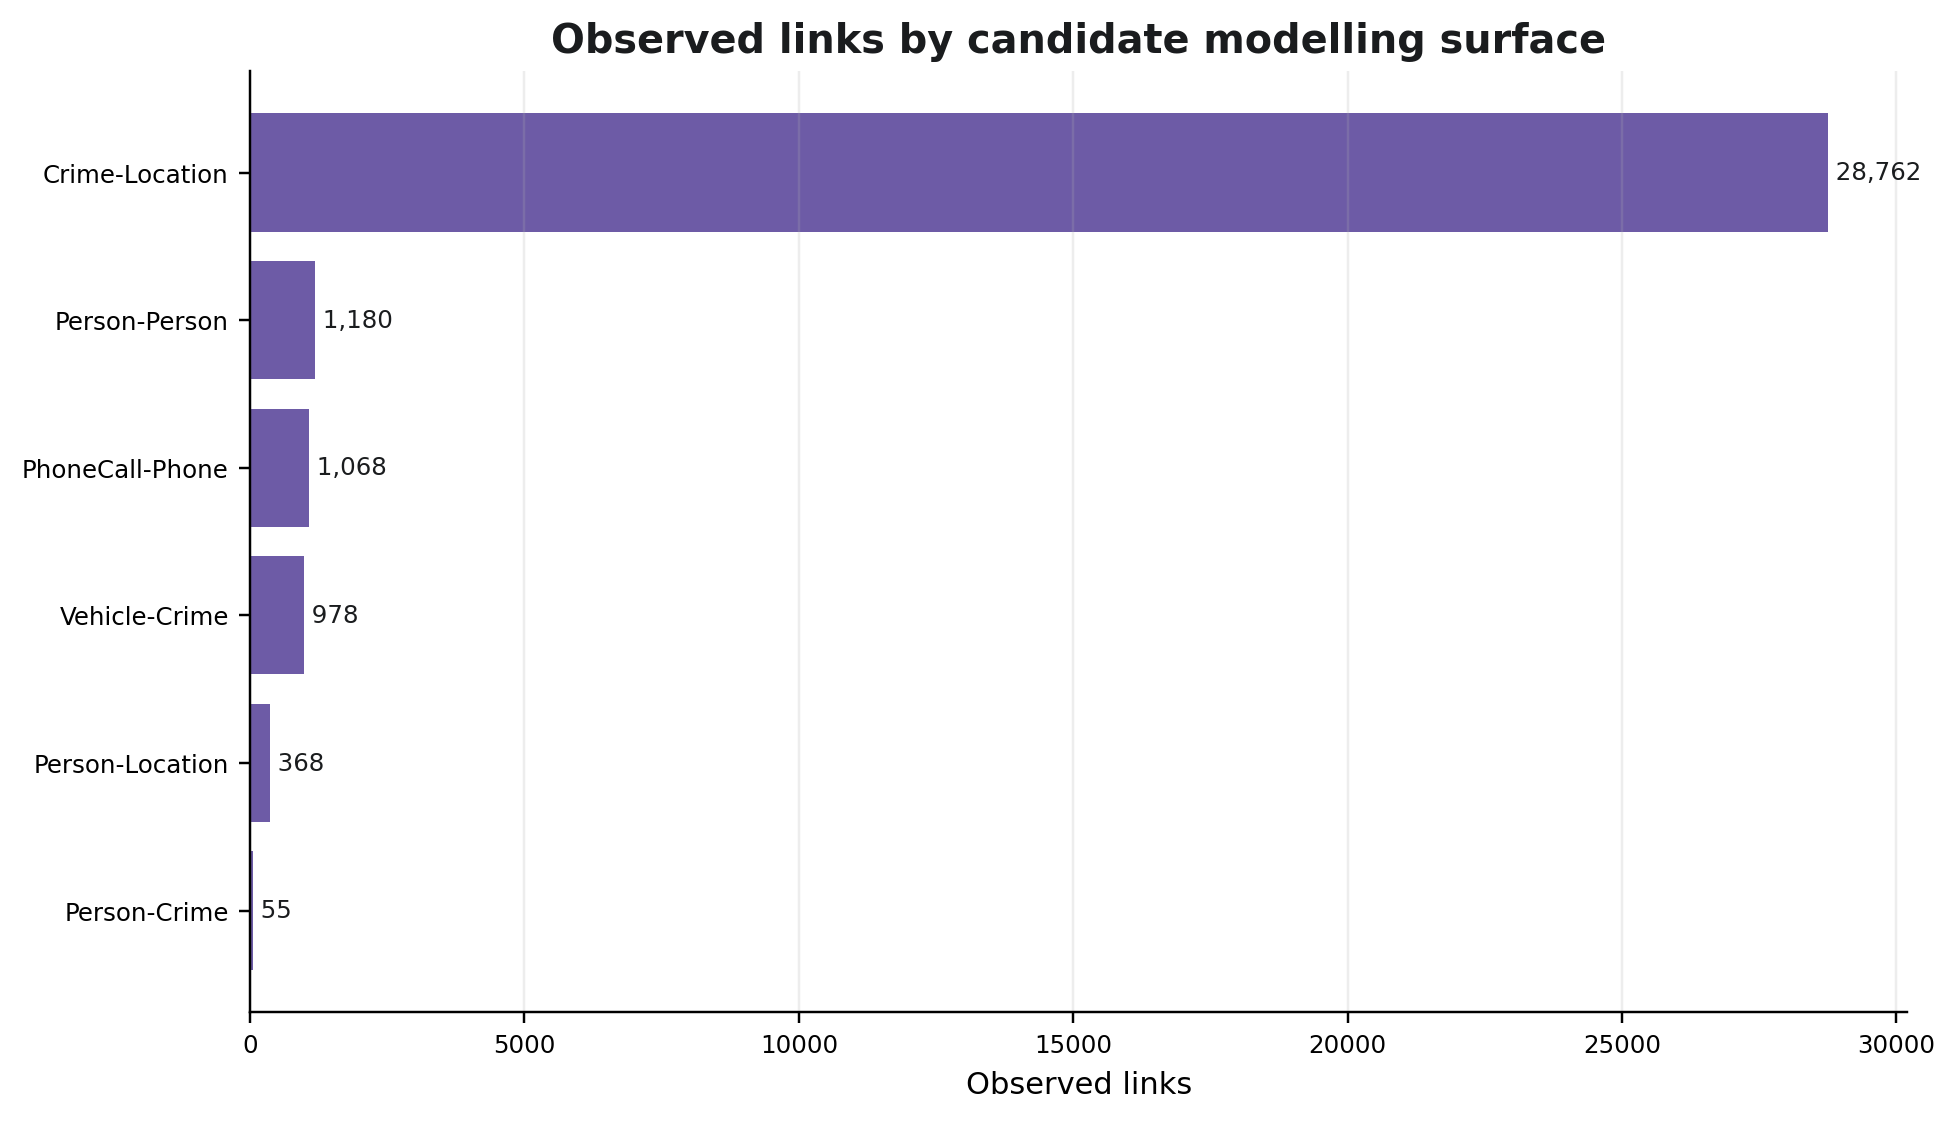
\includegraphics[width=\textwidth,height=0.72\textheight,keepaspectratio]{06_link_viability_counts.png}
  \end{columns}
\end{frame}

\begin{frame}{Graph Stats Result: Specific Place Profiles}
  \small
  \begin{table}
    \centering
    \begin{tabular}{lrlrr}
      \toprule
      \textbf{Place} & \textbf{Total} & \textbf{Dominant type} & \textbf{Type count} & \textbf{Share} \\
      \midrule
      43 Walker's Croft & 35 & Violence and sexual offences & 32 & 91.4\% \\
      182 Waterson Avenue & 35 & Violence and sexual offences & 30 & 85.7\% \\
      109 Soho Street & 20 & Shoplifting & 13 & 65.0\% \\
      135 Barracks Road & 20 & Other crime & 12 & 60.0\% \\
      10 Central Drive & 24 & Violence and sexual offences & 14 & 58.3\% \\
      185 Albion Street & 29 & Violence and sexual offences & 16 & 55.2\% \\
      \bottomrule
    \end{tabular}
  \end{table}

  \vspace{0.1cm}
  This is a better-supported demo claim than individual-level prediction: it is historical, explainable, and directly backed by 28,762 crime-location links.
\end{frame}

\begin{frame}{Graph Stats Result: Concentration and Outcomes}
  \small
  \begin{columns}[T]
    \column{0.48\textwidth}
      \textbf{Place concentration}\\[4pt]
      \begin{tabular}{lr}
        \toprule
        \textbf{Metric} & \textbf{Value} \\
        \midrule
        Crime locations & 12,401 \\
        Total incidents & 28,762 \\
        Top 10 incidents & 3,349 \\
        Top 10 share & 11.6\% \\
        Top 20 share & 13.3\% \\
        \bottomrule
      \end{tabular}

    \column{0.48\textwidth}
      \textbf{Outcome signal}\\[4pt]
      \begin{tabular}{lr}
        \toprule
        \textbf{Outcome} & \textbf{Share} \\
        \midrule
        No suspect identified & 59.4\% \\
        Unable to prosecute & 17.8\% \\
        Under investigation & 11.9\% \\
        Awaiting court & 2.6\% \\
        Local resolution & 1.6\% \\
        \bottomrule
      \end{tabular}
  \end{columns}

  \vspace{0.2cm}
  This gives the report a stronger operational argument: hotspots matter, but outcome difficulty is also central to investigation prioritization.
\end{frame}

\begin{frame}{Graph Stats Result: Operational Difficulty}
  \small
  \begin{table}
    \centering
    \begin{tabular}{lrr}
      \toprule
      \textbf{Crime type} & \textbf{Crimes} & \textbf{Unresolved/no suspect} \\
      \midrule
      Vehicle crime & 2,598 & 95.8\% \\
      Theft from the person & 423 & 95.5\% \\
      Burglary & 2,807 & 94.7\% \\
      Robbery & 541 & 89.8\% \\
      Other theft & 2,140 & 87.1\% \\
      Criminal damage and arson & 3,587 & 81.6\% \\
      Public order & 4,839 & 70.3\% \\
      \bottomrule
    \end{tabular}
  \end{table}

  \vspace{0.1cm}
  These are not ML labels for guilt. They are workload and investigation-difficulty signals that explain why graph triage is useful.
\end{frame}

\begin{frame}{Visual Snapshot: Outcomes and Difficulty}
  \begin{columns}[T]
    \column{0.49\textwidth}
      \centering
      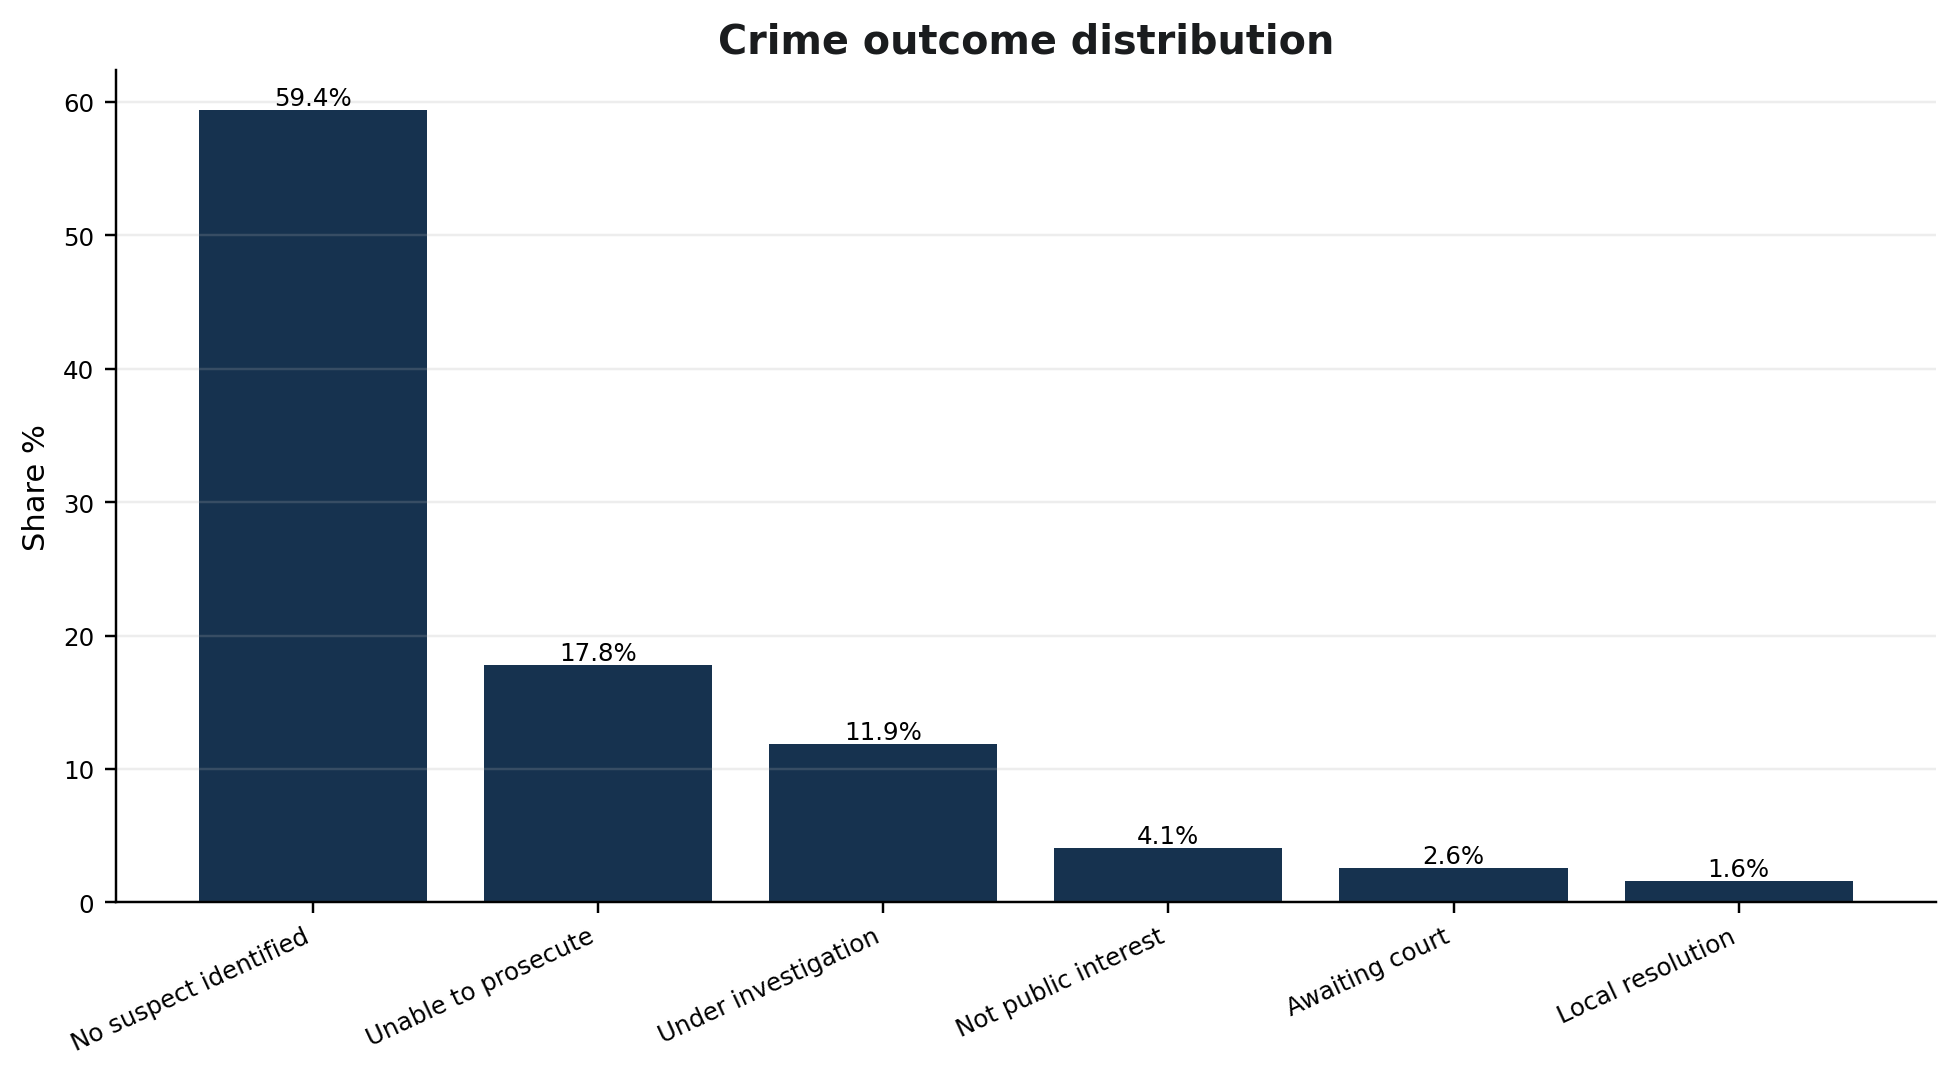
\includegraphics[width=\textwidth,height=0.72\textheight,keepaspectratio]{04_outcome_distribution.png}

    \column{0.49\textwidth}
      \centering
      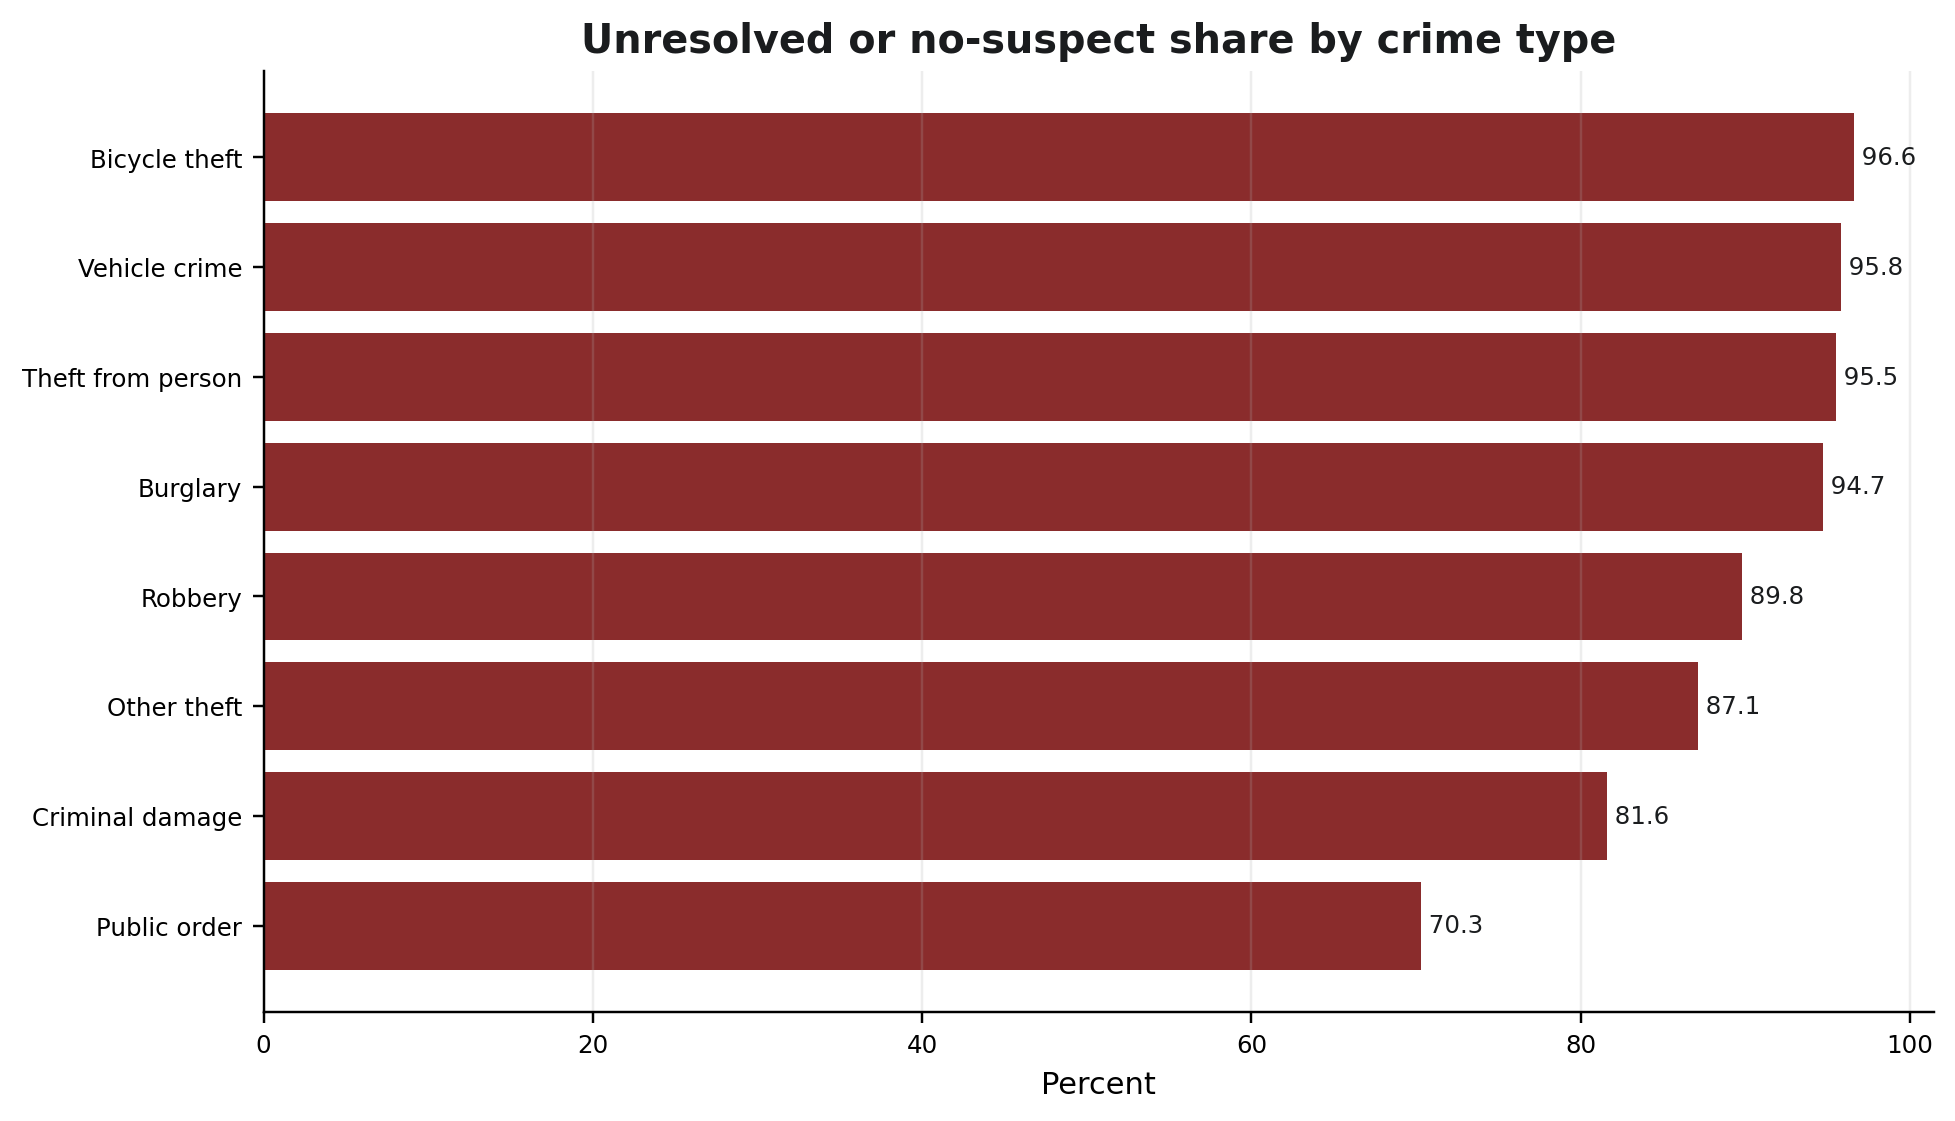
\includegraphics[width=\textwidth,height=0.72\textheight,keepaspectratio]{05_unresolved_by_crime_type.png}
  \end{columns}
\end{frame}

\begin{frame}{Graph Stats Result: Social Communities}
  \begin{columns}[T]
    \column{0.42\textwidth}
      \textbf{Louvain on person social graph}\\[4pt]
      \small
      \begin{tabular}{lr}
        \toprule
        \textbf{Metric} & \textbf{Value} \\
        \midrule
        Person nodes & 369 \\
        Raw social-family relationships & 1,180 \\
        Unique GML target pairs & 586 \\
        Communities & 41 \\
        Modularity & 0.6710 \\
        Reading & Strong \\
        \bottomrule
      \end{tabular}

    \column{0.54\textwidth}
      \textbf{Crime-context concentration}\\[4pt]
      \small
      \begin{tabular}{lrrr}
        \toprule
        \textbf{Community} & \textbf{People} & \textbf{Crime-linked} & \textbf{Share} \\
        \midrule
        239 & 10 & 8 & 80.0\% \\
        237 & 22 & 6 & 27.3\% \\
        331 & 22 & 3 & 13.6\% \\
        226 & 26 & 3 & 11.5\% \\
        351 & 32 & 3 & 9.4\% \\
        \bottomrule
      \end{tabular}
  \end{columns}

  \vspace{0.2cm}
  Reading: Louvain groups people into dense social clusters. Modularity 0.6710 means the social graph has strong community structure, so community-level review is more meaningful than isolated person-crime prediction.
\end{frame}

\begin{frame}{Graph Stats Result: Social Structure Diagnostics}
  \small
  \begin{columns}[T]
    \column{0.48\textwidth}
      \textbf{Structure metrics}\\[4pt]
      \begin{tabular}{lr}
        \toprule
        \textbf{Metric} & \textbf{Value} \\
        \midrule
        Average clustering coefficient & 0.1611 \\
        Weak components & 26 \\
        Largest component & 342 \\
        Maximum k-core & 8 \\
        Phone communication pairs & 118 \\
        Phone pairs already social & 100.0\% \\
        \bottomrule
      \end{tabular}

    \column{0.48\textwidth}
      \textbf{Highest k-core examples}\\[4pt]
      \begin{tabular}{lr}
        \toprule
        \textbf{Person} & \textbf{Core} \\
        \midrule
        Deborah Ford & 8 \\
        Harry Lopez & 8 \\
        Jonathan Hunt & 8 \\
        Peter Bryant & 8 \\
        Phillip Perry & 8 \\
        \bottomrule
      \end{tabular}
  \end{columns}

  \vspace{0.2cm}
  Reading: k-core finds people embedded in tightly connected groups, WCC shows most people sit in one large social component, and phone-call overlap validates that the social layer is not random.
\end{frame}

\begin{frame}{Graph Stats Result: Review-Priority People}
  \small
  \begin{table}
    \centering
    \begin{tabular}{lrrrr}
      \toprule
      \textbf{Person} & \textbf{Own links} & \textbf{Crime neighbours} & \textbf{Address crimes} & \textbf{Score} \\
      \midrule
      Phillip Williamson & 5 & 5 & 1 & 53 \\
      Brian Morales & 4 & 4 & 1 & 46 \\
      Jessica Kelly & 5 & 3 & 1 & 44 \\
      Alan Ward & 3 & 4 & 1 & 40 \\
      Kathleen Peters & 3 & 4 & 2 & 37 \\
      Jack Powell & 4 & 2 & 0 & 31 \\
      Anne Freeman & 0 & 8 & 0 & 26 \\
      \bottomrule
    \end{tabular}
  \end{table}

  \vspace{0.1cm}
  Score = own observed links * 5 + crime-linked neighbours * 2 + neighbour links + address context. This is triage for review, not a conclusion about a person.
\end{frame}

\begin{frame}{Why Person-Crime Prediction Is Not the Main Demo}
  \small
  \begin{table}
    \centering
    \begin{tabular}{lr}
      \toprule
      \textbf{Quantity} & \textbf{Value} \\
      \midrule
      Persons & 369 \\
      Crimes & 28,762 \\
      Possible Person-Crime pairs & 10,613,178 \\
      Observed PARTY\_TO links & 55 \\
      Positive class share & 0.0005\% \\
      \bottomrule
    \end{tabular}
  \end{table}

  \vspace{0.2cm}
  \textbf{Critical decision:} PARTY\_TO remains observed context. It is not used as the final automated write-back target because the class is too sparse and the interpretation is legally sensitive.
\end{frame}

\begin{frame}{Graph ML Design}
  \textbf{Final GML target:} review-only social-family link prediction, with POLE context as features.

  \vspace{0.25cm}
  \begin{columns}[T]
    \column{0.48\textwidth}
      \textbf{Why this is stronger}
      \begin{itemize}
        \item 1,180 raw social-family links collapse into 586 unique undirected pair labels, not 55 \tinycode{PARTY\_TO} labels.
        \item Safer interpretation: candidate association, not a crime claim.
        \item Social graph has meaningful Louvain structure.
      \end{itemize}

    \column{0.48\textwidth}
      \textbf{Context graph}
      \begin{itemize}
        \item Person, Phone, Email, Location, Crime.
        \item Social links, address links, contact links.
        \item PARTY\_TO and OCCURRED\_AT retained only as context.
      \end{itemize}
  \end{columns}
\end{frame}

\begin{frame}{Supervised GDS Pipeline}
  \small
  \begin{table}
    \centering
    \begin{tabular}{p{0.28\textwidth}p{0.58\textwidth}}
      \toprule
      \textbf{Stage} & \textbf{Choice} \\
      \midrule
      Projection & \tinycode{socialFamilyContextGraph} over Person/Crime/Location/Phone/Email context, with the supervised target handled separately for train/test splitting. \\
      Target & Unified undirected social-family Person--Person pairs derived from raw social-family relationship evidence. \\
      Embedding & FastRP 128 dimensions and Node2Vec 64 dimensions. \\
      Pair feature & Hadamard product of source and target embeddings. \\
      Models & Logistic Regression and Random Forest candidates. \\
      Selection & GDS chooses the best candidate by validation AUCPR, then reports held-out test AUCPR. \\
      Metric & AUCPR because the positive class is sparse. \\
      Deployment & Write-back gate requires acceptable held-out AUCPR and probability spread. \\
      \bottomrule
    \end{tabular}
  \end{table}
\end{frame}

\begin{frame}{Expanded ML Strategy}
  \small
  \begin{table}
    \centering
    \begin{tabular}{p{0.28\textwidth}p{0.23\textwidth}p{0.35\textwidth}}
      \toprule
      \textbf{Strategy} & \textbf{Result} & \textbf{Interpretation} \\
      \midrule
      Supervised social LP & RF selected, test AUCPR 0.5578 & Useful for ranking rare candidate links; 25 review-only candidates written. \\
      Explainable social LP & 4 review links & Strongest auditable GML output. \\
      FastRP + kNN & high-similarity candidate pairs & Unsupervised review queue, no labels required. \\
      Crime-type classification & F1 0.1441, accuracy 0.3096 & Weak supervised result; graph context alone does not reliably recover crime type. \\
      Hotspot analytics & 28,762 location links & Strongest operational insight. \\
      \bottomrule
    \end{tabular}
  \end{table}

  \vspace{0.1cm}
  This is the key upgrade: multiple strategies are tested, and weak models become evidence for limits rather than hidden failures.
\end{frame}

\begin{frame}{Visual Snapshot: Model Comparison}
  \begin{columns}[T]
    \column{0.56\textwidth}
      \centering
      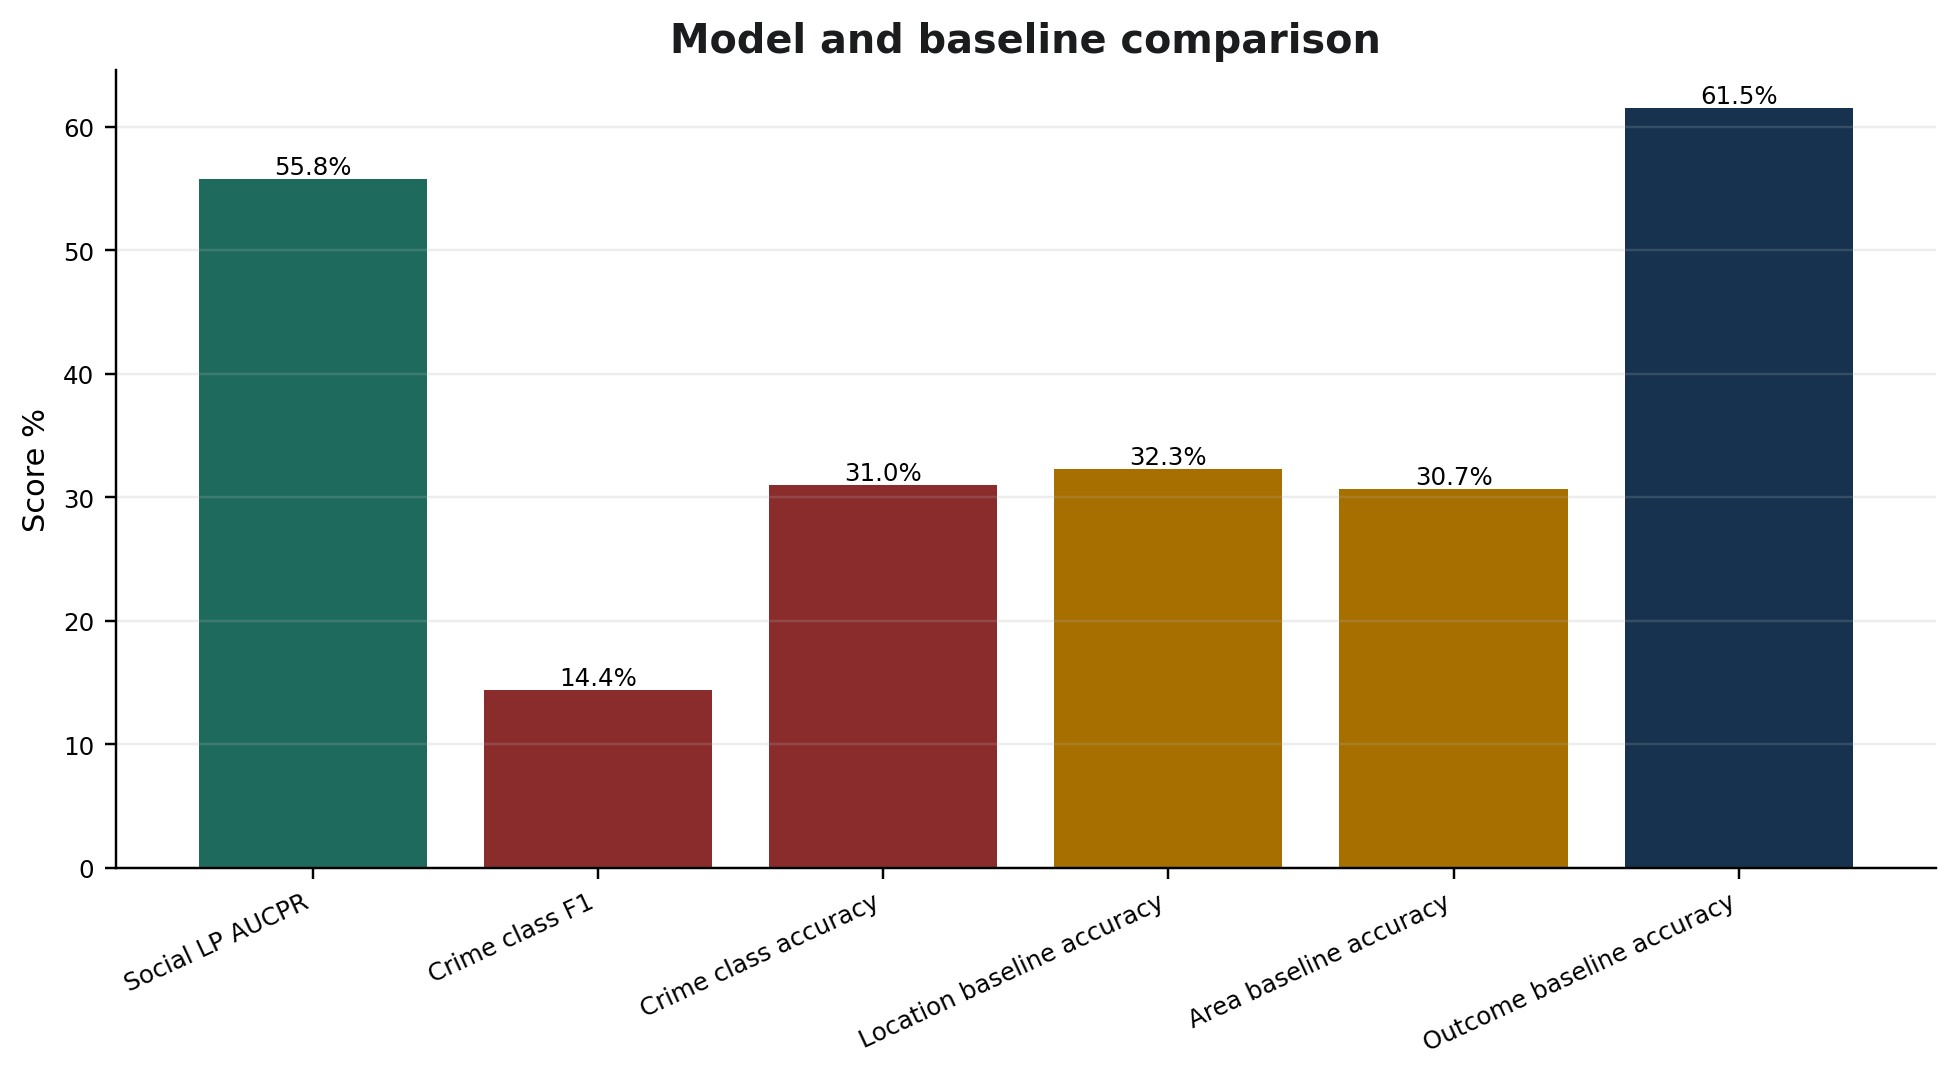
\includegraphics[width=\textwidth,height=0.72\textheight,keepaspectratio]{07_model_baseline_comparison.png}

    \column{0.40\textwidth}
      \centering
      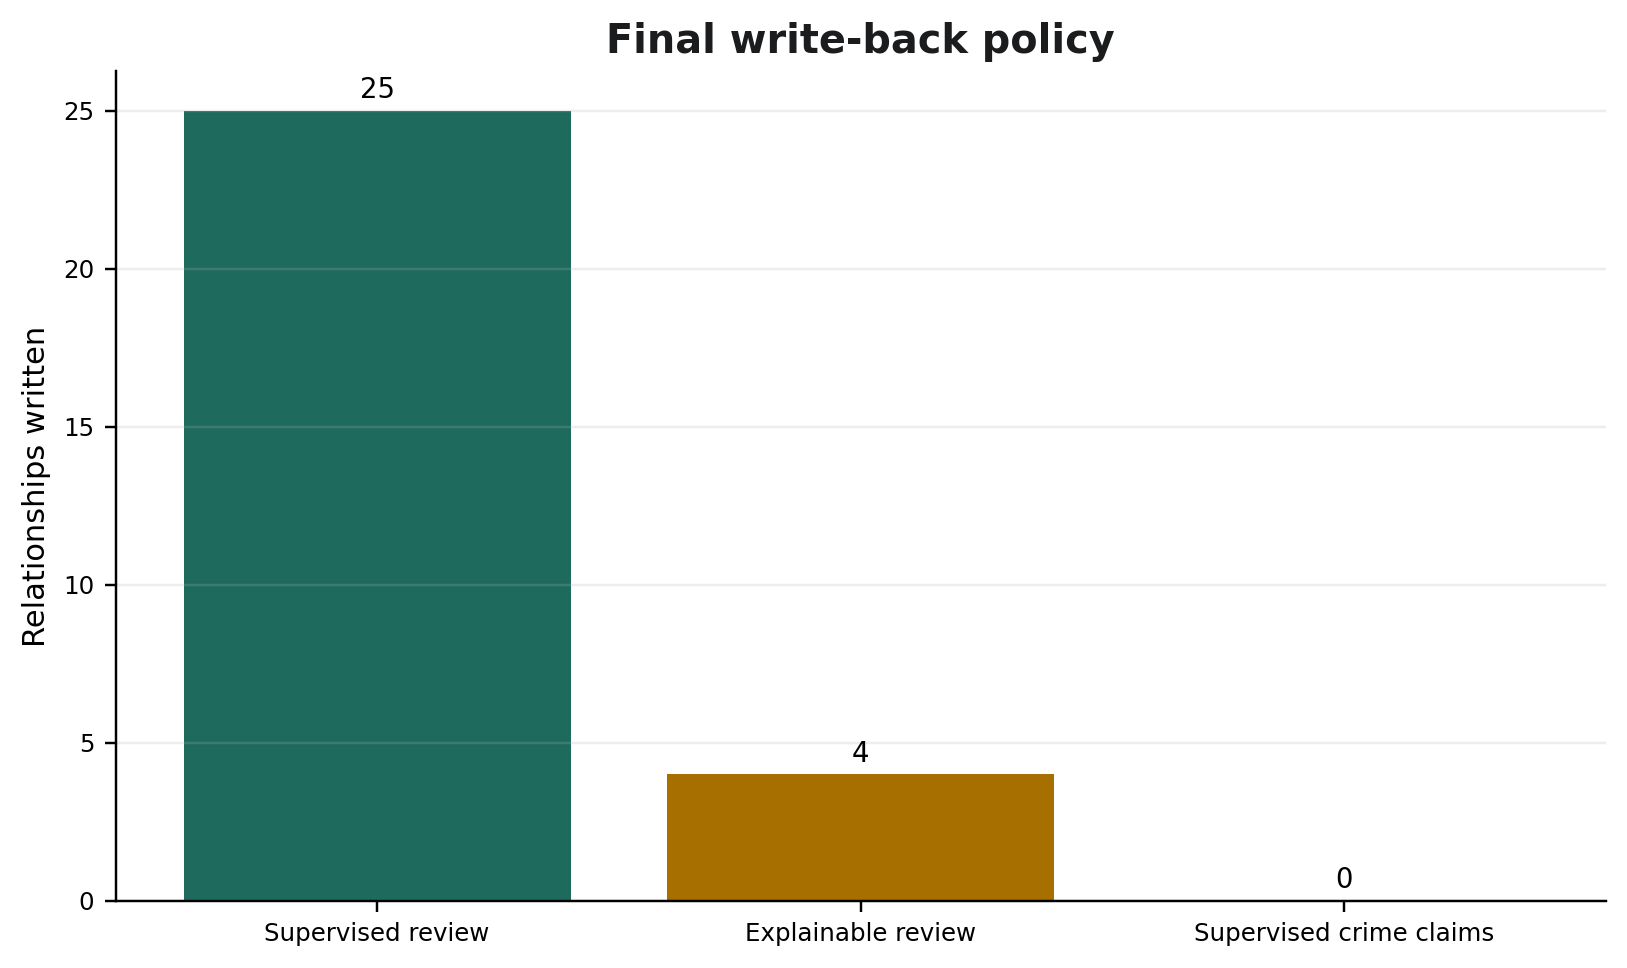
\includegraphics[width=\textwidth,height=0.72\textheight,keepaspectratio]{08_writeback_policy.png}
  \end{columns}
  \small
Note: this is a diagnostics dashboard, not a single leaderboard. AUCPR, F1, and accuracy answer different evaluation questions.
\end{frame}

\begin{frame}{Main Metrics}
  \small
  \begin{table}
    \centering
    \begin{tabular}{p{0.22\textwidth}p{0.28\textwidth}p{0.36\textwidth}}
      \toprule
      \textbf{Metric} & \textbf{Plain meaning} & \textbf{How we use it} \\
      \midrule
      AUCPR & Ranking quality for rare positive links & Main score for social-family link prediction. \\
      Weighted F1 & Balance of precision and recall across classes & Used for crime-type classification; low score means not deployed. \\
      Louvain modularity & Strength of community separation & 0.6710 supports community-level analysis. \\
      k-core & How deeply a person sits inside a connected group & Used for social-structure diagnostics, not accusation. \\
      Probability spread & Whether candidate scores are meaningfully separated & Used as a deployment gate before write-back. \\
      \bottomrule
    \end{tabular}
  \end{table}
\end{frame}

\begin{frame}{Supervised Link Prediction Metrics}
  \begin{columns}[T]
    \column{0.46\textwidth}
      \textbf{Target density}\\[4pt]
      \small
      \begin{tabular}{lr}
        \toprule
        \textbf{Metric} & \textbf{Value} \\
        \midrule
        People & 369 \\
        Unique social-family target pairs & 586 \\
Candidate directed person pairs & 135,792 \\
Positive share over directed pairs & 0.4315\% \\
        \bottomrule
      \end{tabular}
      \vspace{0.1cm}
\scriptsize
The supervised target is deduplicated as person-pair evidence; candidate scoring is reported over directed source-target pairs from the GDS pipeline.

    \column{0.50\textwidth}
      \textbf{GDS model-comparison result}\\[4pt]
      \small
      \begin{tabular}{lr}
        \toprule
        \textbf{Metric} & \textbf{Value} \\
        \midrule
        Selected model & Random Forest \\
        Train AUCPR & 0.8034 \\
        Validation AUCPR & 0.6271 \\
        Test AUCPR & 0.5578 \\
        \bottomrule
      \end{tabular}

      \vspace{0.25cm}
      Reading: AUCPR measures how well the model ranks rare true links above non-links. A test AUCPR of 0.5578 is useful for review-priority ranking, but not strong enough for automatic decisions.
  \end{columns}
\end{frame}

\begin{frame}{Why AUCPR and Calibration Matter}
  \small
  The course asks for graph machine learning results, but the useful result is not just the model score. The deployment decision matters too.

  \vspace{0.2cm}
  \begin{table}
    \centering
    \begin{tabular}{p{0.28\textwidth}p{0.56\textwidth}}
      \toprule
      \textbf{Question} & \textbf{Answer from final results} \\
      \midrule
      Is the target imbalanced? & Yes. Social-family positives are only 0.4315\% of directed person pairs. \\
      Is accuracy meaningful? & No. A no-link baseline would look accurate but would learn nothing useful. \\
      Is AUCPR more appropriate? & Yes. It focuses on rare positive links and ranking quality. \\
      Is the trained model deployable? & Only as review support. Random Forest was selected by validation AUCPR and held-out test AUCPR is 0.5578. \\
      What is the responsible result? & Write review-only candidates, keep explanations, and avoid crime accusations. \\
      \bottomrule
    \end{tabular}
  \end{table}
\end{frame}

\begin{frame}{Calibration Result}
  \small
  \begin{table}
    \centering
    \begin{tabular}{lr}
      \toprule
      \textbf{Deployment gate output} & \textbf{Value} \\
      \midrule
      Selected supervised model & Random Forest \\
      Held-out test AUCPR & 0.5578 \\
      Candidate social links scored & 130 \\
      Lowest probability & 0.70 \\
      Highest probability & 0.885 \\
      Average probability & 0.7449 \\
      Probability band & 0.18 \\
      Supervised write-back links & 25 \\
      \bottomrule
    \end{tabular}
  \end{table}

  \vspace{0.2cm}
  Reading: probabilities are treated as ranking scores, not truth claims. The gate writes only the top review-only social candidates when the model has acceptable held-out AUCPR and a non-flat probability spread.
\end{frame}

\begin{frame}{Unsupervised Similarity Result}
  \small
  \begin{table}
    \centering
    \begin{tabular}{llr}
      \toprule
      \textbf{Person A} & \textbf{Person B} & \textbf{Similarity} \\
      \midrule
      Daniel Moreno & Mary Peters & 1.0000 \\
      Heather Howard & Jennifer Jacobs & 1.0000 \\
      Heather Howard & Maria Rivera & 1.0000 \\
      Jennifer Jacobs & Maria Rivera & 1.0000 \\
      Joseph Rogers & Peter Burns & 1.0000 \\
      Anne Clark & Jerry Fernandez & 0.9786 \\
      Nancy Hughes & Larry Turner & 0.9715 \\
      \bottomrule
    \end{tabular}
  \end{table}

  \vspace{0.1cm}
  Reading: FastRP turns each person’s graph neighbourhood into a vector, and kNN finds people with similar graph context. These are similarity candidates, not predicted crimes.
\end{frame}

\begin{frame}{Secondary Supervised Task: Crime Type Classification}
  \small
  \begin{table}
    \centering
    \begin{tabular}{lr}
      \toprule
      \textbf{Metric} & \textbf{Value} \\
      \midrule
      Graph projection & Crime, Location, Officer, Vehicle, Object \\
      Relationships & OCCURRED\_AT, INVESTIGATED\_BY, INVOLVED\_IN \\
      Embedding & FastRP, 32 dimensions \\
      Model & Logistic Regression \\
      Test weighted F1 & 0.1441 \\
      Test accuracy & 0.3096 \\
      \bottomrule
    \end{tabular}
  \end{table}

  \vspace{0.1cm}
  Reading: weighted F1 balances performance across crime classes. A score of 0.1441 is weak, so this task becomes evidence that graph context helps triage more than it predicts crime type.
\end{frame}

\begin{frame}{Deployment Sanity Check}
  \small
For newly predicted candidate links, true labels are not available at demo time. So we separate model evaluation from deployment: AUCPR evaluates held-out known links, while the write-back table shows what the deployed pipeline actually outputs.
  \vspace{0.2cm}
  \begin{table}
    \centering
    \begin{tabular}{lrr}
  \toprule
  \textbf{Deployment decision} & \textbf{Count} & \textbf{Interpretation} \\
  \midrule
  Written as review-only social candidate & 25 & Needs human validation \\
  Held for no write-back & 105 & Not selected by the conservative top-25 write-back gate \\
  \bottomrule
\end{tabular}
  \end{table}

  \vspace{0.2cm}
  \textbf{Operational metric:} overclaiming risk is controlled by writing review-only social candidates, not crime claims. Model quality is reported with AUCPR; deployment quality is reported with probability spread and write-back count.
\end{frame}

\begin{frame}{Baseline Confusion Matrix for Class Imbalance}
  \small
  For the social-family target evaluated over directed candidate pairs, naive baselines are misleading:

  \vspace{0.2cm}
  \begin{table}
    \centering
    \begin{tabular}{lrrr}
      \toprule
      \textbf{Baseline} & \textbf{TP} & \textbf{FP} & \textbf{FN} \\
      \midrule
      Predict no links & 0 & 0 & 586 \\
      Predict all directed pairs as links & 586 & 135,206 & 0 \\
      \bottomrule
    \end{tabular}
  \end{table}

  \vspace{0.2cm}
  The no-link baseline has 99.5685\% accuracy but zero recall, so it misses every true social-family pair. That is why AUCPR and review-gated write-back are more honest than accuracy.
\end{frame}

\begin{frame}{Explainable GML Baseline: Common Neighbours}
  \small
  \begin{table}
    \centering
    \begin{tabular}{lll}
      \toprule
      \textbf{Person A} & \textbf{Person B} & \textbf{Shared neighbours} \\
      \midrule
      Amanda Alexander & Kathryn Allen & 3 \\
      Jessica Kelly & Alan Ward & 3 \\
      Roy Dean & Harry Lopez & 3 \\
      Roy Dean & Jonathan Hunt & 3 \\
      \bottomrule
    \end{tabular}
  \end{table}

  \vspace{0.2cm}
  These are easy to explain live: two people are candidates only when they share multiple specific neighbours and have no existing social edge.
\end{frame}

\begin{frame}{Explainable GML Baseline: Adamic Adar}
  \small
  \begin{table}
    \centering
    \begin{tabular}{llrl}
      \toprule
      \textbf{Person A} & \textbf{Person B} & \textbf{AA score} & \textbf{Explanation} \\
      \midrule
      Jessica Kelly & Alan Ward & 1.2710 & Brian Morales, Phillip Williamson, Kathy Wheeler \\
      Amanda Alexander & Kathryn Allen & 1.2490 & Benjamin Hamilton, Denise Brown, Wanda Webb \\
      Roy Dean & Harry Lopez & 1.1506 & shared specific neighbours \\
      Roy Dean & Jonathan Hunt & 1.1506 & shared specific neighbours \\
      Amy Murphy & Ann Fox & 0.9605 & Justin Arnold, Jessica Kelly \\
      \bottomrule
    \end{tabular}
  \end{table}

  \vspace{0.2cm}
  Reading: Adamic Adar gives more weight to rare shared neighbours, so the explanation is stronger when two people share specific, less-common contacts. Final write-back: 4 \tinycode{PREDICTED\_SOCIAL\_EXPLAINABLE} links, all review-only.
\end{frame}

\begin{frame}{Final GML Decision Table}
  \small
  \begin{table}
    \centering
    \begin{tabular}{p{0.28\textwidth}p{0.2\textwidth}p{0.38\textwidth}}
      \toprule
      \textbf{Approach} & \textbf{Result} & \textbf{Decision} \\
      \midrule
      Person-Crime prediction & 55 labels, 0.0005\% positives & Keep as context only. Too sparse and sensitive. \\
      Supervised social LP & Random Forest selected; test AUCPR 0.5578 & Used as ranking support; 25 review-only candidates written. \\
      FastRP + kNN & Similarity candidates up to 1.0000 & Unsupervised review queue. \\
      Crime-class classifier & Test weighted F1 0.1441 & Negative supervised result, not deployed. \\
      Common Neighbours / Adamic Adar & 4 high-specificity links & Strongest explainable GML output, written as review-only. \\
      Hotspot analytics & 28,762 complete crime-location links & Main investigative insight. \\
      Community analytics & Louvain modularity 0.6710 & Main graph-structure insight. \\
      \bottomrule
    \end{tabular}
  \end{table}
\end{frame}

\begin{frame}{Comparative Insight}
  \begin{columns}[T]
    \column{0.48\textwidth}
      \textbf{Conventional ML framing}
      \begin{itemize}
        \item Needs labelled rows.
        \item Struggles when the target has only 55 positives.
        \item Harder to explain multi-hop context.
      \end{itemize}

    \column{0.48\textwidth}
      \textbf{Graph ML framing}
      \begin{itemize}
        \item Uses paths, neighbours, communities, and structural similarity.
        \item Can produce human-readable explanations.
        \item Still needs calibration before deployment.
      \end{itemize}
  \end{columns}

  \vspace{0.3cm}
  Final position: GDS is strongest here as an investigative prioritization layer, not as an automated decision engine.
\end{frame}

\begin{frame}{Live Demo Script}
  \begin{enumerate}
    \item Show database model and counts: \tinycode{CALL db.schema.visualization()} and graph stats schema queries.
    \item Run link viability audit to prove which relationships are strong.
    \item Run hotspot query: top repeat locations and dominant crime type.
    \item Run Louvain community query and community crime-context concentration.
    \item Run supervised social-family pipeline metrics and calibration query.
    \item Show four review-only \tinycode{PREDICTED\_SOCIAL\_EXPLAINABLE} links and their shared-neighbour explanations.
    \item Close with the final conclusion query.
  \end{enumerate}
\end{frame}

\begin{frame}{Submission Notes}
  \begin{itemize}
    \item Final demo script is reproducible from \tinycode{graph-stats/queries.cypher} and \tinycode{graph-ml/pipeline.cypher}.
    \item Result evidence is saved in \tinycode{graph-stats/results.cypher} and \tinycode{graph-ml/results.cypher}.
    \item Local Neo4j credentials are stored only in an ignored local config file and are not part of submission.
    \item Generative AI was used as an assistant for debugging, wording, and code/result review. Final modelling choices, interpretation, and demo claims remain the team's responsibility.
    \item The final paper can reuse the same structure: problem, graph design, stats/analytics, GML methodology, results, limitations, and conclusion.
  \end{itemize}
\end{frame}

\begin{frame}{Limitations and Ethics}
  \begin{itemize}
    \item Sparse labels make direct person-crime prediction unreliable as a deployed target.
    \item Historical hotspots are not causal forecasts.
    \item Address exposure and social proximity are context only.
    \item The model writes no automated crime claims.
    \item Human review is required before any investigative action.
    \item Final claims are backed by the saved Cypher scripts and result files.
  \end{itemize}
\end{frame}

\begin{frame}{Final Results}
  \small
  \begin{table}
    \centering
    \begin{tabular}{lr}
      \toprule
      \textbf{Final result} & \textbf{Value} \\
      \midrule
      Crime-location links powering hotspot analysis & 28,762 \\
      Raw social links powering community analysis & 1,180 \\ 
      Unique social-family pairs for GML target & 586 \\
      Louvain communities & 41 \\
      Louvain modularity & 0.6710 \\
      Supervised social selected model & Random Forest \\
      Supervised social test AUCPR & 0.5578 \\
      Supervised review-only links & 25 \\
      Crime-class test weighted F1 & 0.1441 \\
      Explainable review-only links written & 4 \\
      Person-Crime links used as context only & 55 \\
      \bottomrule
    \end{tabular}
  \end{table}

  \vspace{0.2cm}
  The final results are more convincing because they use the dense, explainable parts of the POLE graph instead of forcing the weakest target to carry the whole project.
\end{frame}

\begin{frame}{Final Evidence Scorecard}
  \centering
  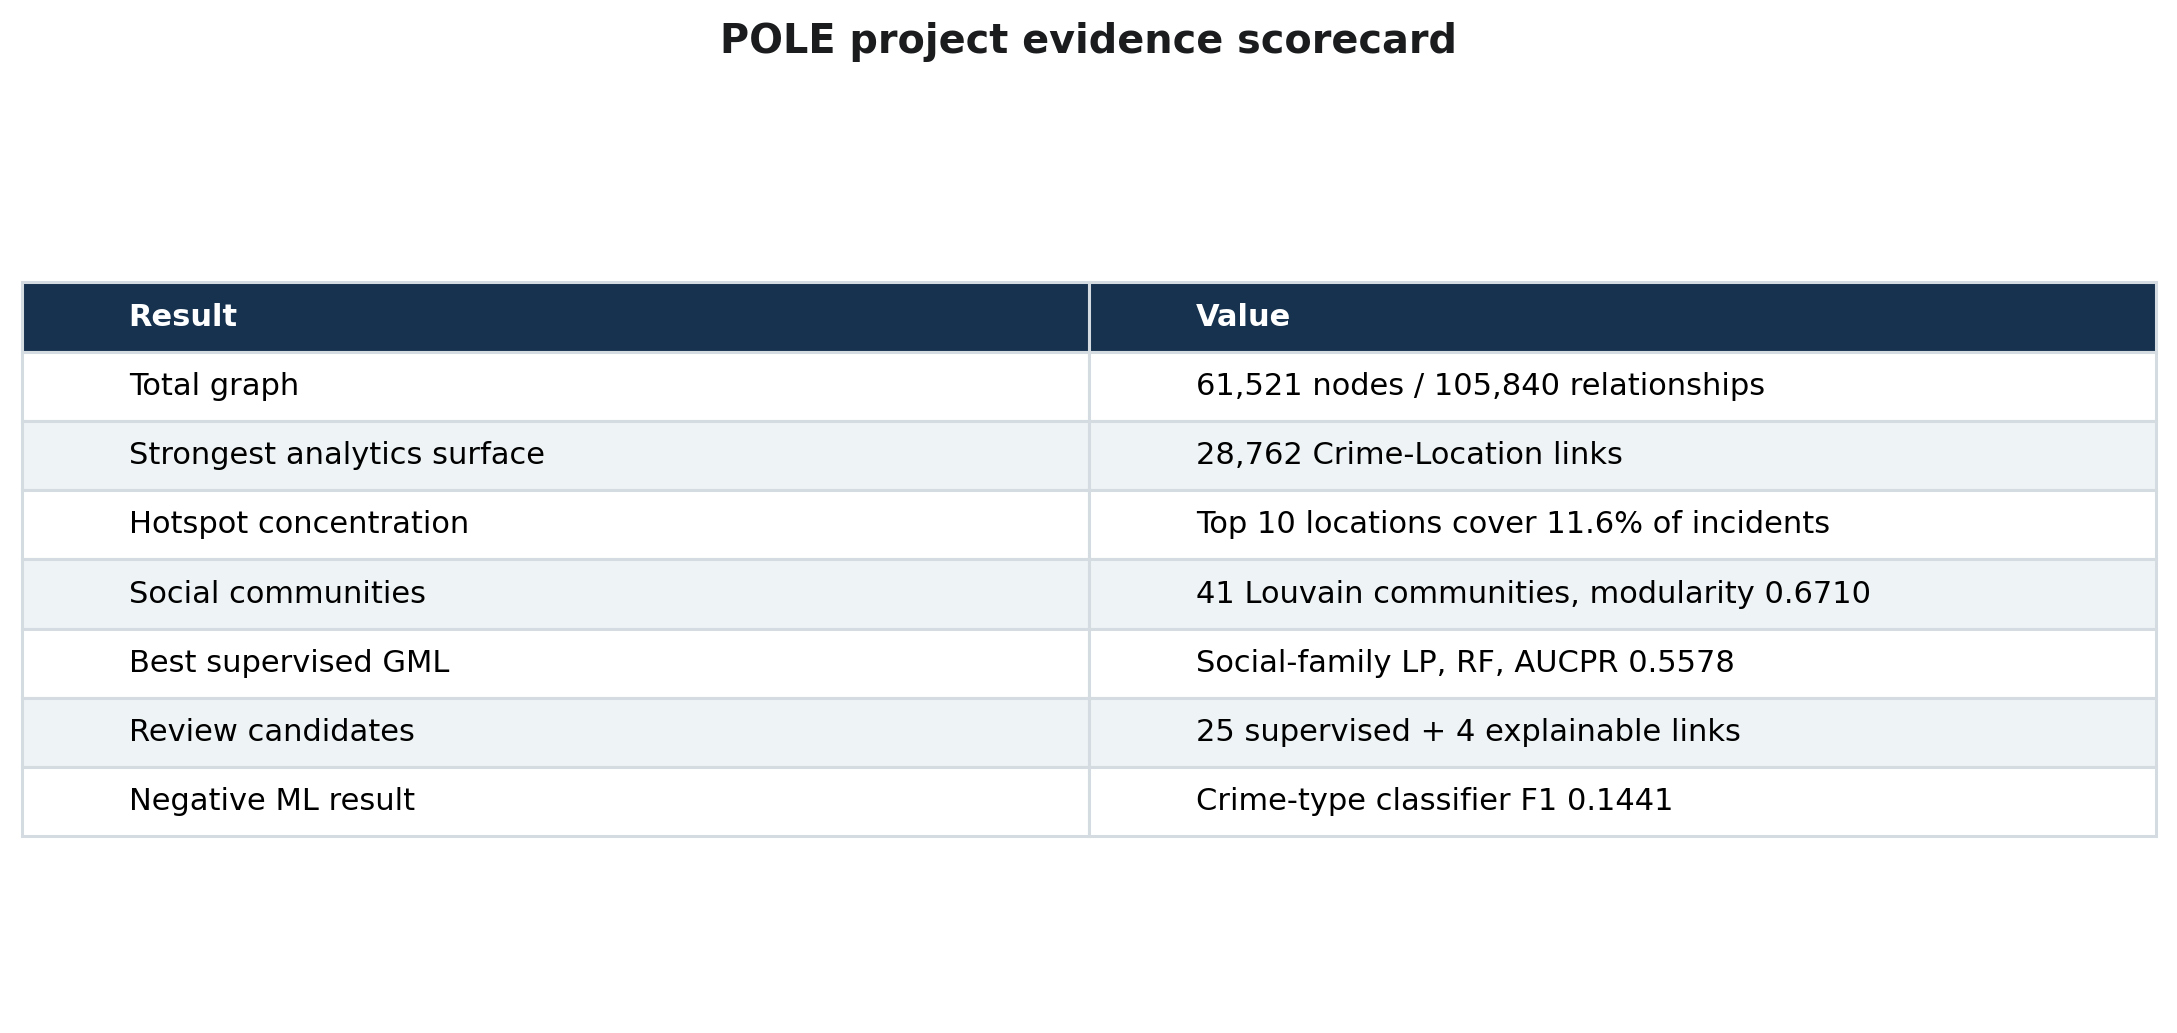
\includegraphics[width=0.92\textwidth,height=0.78\textheight,keepaspectratio]{09_project_scorecard.png}
\end{frame}

\begin{frame}{Final Takeaway}
  \begin{block}{Project conclusion}
    The strongest final demo is POLE investigative analytics: hotspot locations, community concentration, review-priority people, and explainable social-link candidates. Direct Person-Crime prediction was tested, but the evidence base was too sparse for automated write-back.
  \end{block}

  \vspace{0.25cm}
  \textbf{One-line demo message:} We did not just build a model; we built a graph workflow that selects safe targets, explains its outputs, and knows when not to trust the model.
\end{frame}

\begin{frame}
  \vfill
  \centering
  {\Huge\color{Navy} Questions?}
  \vfill
\end{frame}

\end{document}

